% *************************************************************************
% *    IWI Hamburg / Prof. Dr. Stefan Voß
% *    Thesis / Dissertation Latex Template                                        
% *    
% *    Author: Leonard Heilig <leonard.heilig@uni-hamburg.de>
% *   
% *    Note: some parts of this template are based on the VSIS template
% *              of Michael von Riegen <riegen@informatik.uni-hamburg.de>
% *   
% *************************************************************************

\documentclass[
      paper=a4,
      12pt,
      twoside=false,
      openright,
]{scrbook}



% DEFINE THESIS SETTINGS
% Bitte füllen Sie die folgenden Daten vollständig aus
\newcommand\myName{Max Mustermann}
\newcommand\myAddress{Musterstr. 7e, 22529 Hamburg}
\newcommand\myEmail{max.mustermann@studium.uni-hamburg.de}
\newcommand\myKeywords{<...>} % Optional
\newcommand\myMatNr{<...>}
\newcommand\myTitle{Titel}
\newcommand\myShortTitleForHeader{Kurztitel}
\newcommand\thesisType{<Expos\'{e} / Bachelorarbeit / Masterarbeit>}
\newcommand\faculty{<...>} % z.B. MIN-Fakultät
\newcommand\fachbereich{} % Optional: z.B. Fachbereich Informatik
\newcommand\courseOfStudies{<...>}
\newcommand\supervisor{<Name des Betreuers>}
\newcommand\primaryReferee{<Name des Erstgutachters>}
\newcommand\primaryRefereeInst{<Institute of Information Systems>}
\newcommand\secondaryReferee{<Name des Zweitgutachters>}
\newcommand\secondaryRefereeInst{<Name des Instituts>}
\newcommand\optionalQuote{} % shown after title page

\title{\mytitle}
\author{\myName \\ \texttt{\myEmail}}

% IMPORT PACKAGES AND SETTINGS
\usepackage{settings}





% ************ DOCUMENT BEGINS

\begin{document}

    % CHOOSE "ngerman" or "english"
    \selectlanguage{ngerman}
    
    % Please change this part to _titlepage_en for the English version
    % *************************************************************************
% *    IWI Hamburg / Prof. Dr. Stefan Voß
% *    Thesis / Dissertation Latex Template                                        
% *    
% *    Author: Leonard Heilig <leonard.heilig@uni-hamburg.de>
% *   
% *    Note: some parts of this template are based on the VSIS template
% *              of Michael von Riegen <riegen@informatik.uni-hamburg.de>
% *   
% *************************************************************************

\begin{titlepage}

% START PAGE: -1
\setcounter{page}{-1}    

\begin{figure}[h]
    
     \begin{flushleft}
     	
     \end{flushleft}
     \hspace{-40px}
     \noindent\begin{minipage}[t][0px][b]{0.3\textwidth}
     	%\noindent
\includegraphics[width=8cm,clip]{images/up-uhh-logo-u-2010-u-png}
     	\noindent
\includegraphics[scale=0.3]{images/UHH-Logo_2010_Farbe_CMYK.pdf}
     \end{minipage}
     \hspace{50px}
     \begin{flushright}
     	
     	\begin{minipage}[t][-70px][b]{0.38\textwidth}
     		\begin{flushright}
     			\sffamily{
     			%	{\small \textbf{Institute of Information Systems} } \\
     			%	\small Prof. Dr. Stefan Voß \\
     			}
     		\end{flushright}
     	\end{minipage}
     	\hspace{5px}
     	\begin{minipage}[t][-47px][b]{0.14\textwidth}
     	%	
\includegraphics[width=2cm,clip]{images/IWI_logo}
     	\end{minipage}
     \end{flushright}
     

    
\end{figure}

\vfill
\vspace{10mm}

\large
\begin{center}

    % THESIS TYPE
	\noindent { 
	 \color{uhhred}\textbf{\MakeUppercase \thesisType}
	}
	\vspace{2.0cm}\\
	% THESIS TITLE
	\textbf{\Large \myTitle} 
	\vspace{2.0cm}\\ presented by
\vspace{0.4cm}\\
\myName
	
\end{center}
	
\vfill

\begin{tabbing}
	\hspace{10em} \=  \kill
	%Presented by: \> \textbf{\myName} \\
	%\> \textrm{\myAddress} \\
	%\> \textrm{\myEmail} \\ 
	Faculty: \>  \faculty \\
	\> \fachbereich \\
	Course of Studies: \>  \courseOfStudies \\ %~(Semester \currentSemester)
	Matriculation Number: \>  \myMatNr \\ \\
	Supervisor: \> \supervisor \\
	Primary Referee: \> \primaryReferee \\
	 \>	\primaryRefereeInst \\
	Secondary Referee: \> \secondaryReferee \\
	 \>	\secondaryRefereeInst \\
	%Date of submission: \> \dateOfSubmission \\
\end{tabbing}


% BLANK PAGE WITH A QUOTE (OPTIONAL)
\newpage 
	
\thispagestyle{empty}
\setcounter{page}{0}

~\\ \vfill \noindent 
\optionalQuote

\end{titlepage}

\renewcommand{\cfttabpresnum}{Tab. } 
\renewcommand{\cftfigpresnum}{Fig. } 
\renewcommand{\nomname}{List of Abbreviations}
\renewcommand{\contentsname}{List of Contents}
\renewcommand{\listfigurename}{List of Figures}
\renewcommand{\listtablename}{List of Tables}


    \frontmatter  % ROMAN NUMBERING              
    %\textbf{Stichwörter :} \myKeywords
\subsubsection{Abstract}



	
    \tableofcontents
    
    \listoffigures
    \addcontentsline{toc}{chapter}{\listfigurename}
    
    \listoftables
    \addcontentsline{toc}{chapter}{\listtablename}
    

    % LIST OF ABBREVIATIONS
    \makenomenclature
    \printnomenclature[9em]

    \mainmatter % ARABIC NUMBERING            

    % INCLUDE TEX CHAPTERS
    \chapter{Introduction}

\lipsum[2] Meanwhile, information technology~(IT)\nomenclature{IT}{Information technology} has become essential to exchange information between involved inter-organizational actors and across global supply chains more efficiently. Big data can be defined as ``data whose size forces us to look beyond the tried-and-true methods that are prevalent at that time.'' \citep[][p.~44]{jacobs_pathologies_2009}


Although a consistent definition of big data has yet to be specified, there is a common understanding that big data is data whose size and complexity forces us to look beyond conventional tools and methods to exploit and utilize it \citep[cf.][p.~44]{jacobs_pathologies_2009}.

According to \citet[][p.~44]{jacobs_pathologies_2009},  big data can be seen as data whose size $e + p = y$ and complexity forces us to look beyond conventional tool and methods to exploit and utilize it. 

\begin{compactitem}
	\item \citet{fink2006grundlagen} 
	\item \citet{bose2000vehicle} 
	\item \citet{heilig_scientometric_2014} 
	\item \citet{voss_popmusic_2002} 
	\item \citet{davenport_data_2012}
	\item \citet{ropke_heuristic_2005}
	\item \citet{heilig_voss_2015}
\end{compactitem}

\lipsum[2]



\vspace{10pt}
\begin{table}[H]
	\centering
	  \renewcommand{\arraystretch}{1.5}
		\begin{tabular}{p{3.5cm}p{10.5cm}l}
		\toprule
 On-demand \mbox{self-service} & \lipsum[1]
 \\\midrule
 Elasticity \mbox{and scalability} & \lipsum[1]
\\\bottomrule
 \end{tabular}
	\caption[Key characteristics of cloud computing]{Key characteristics of cloud computing \citep{armbrust2010view}}
	\label{tab:cloud.characteristics}
	
\end{table}
    \chapter{Kapitel}

\section{Unterkapitel}

\subsection{Unterunterkapitel}

\lipsum[2]

\begin{figure}[h!]
	\centering
		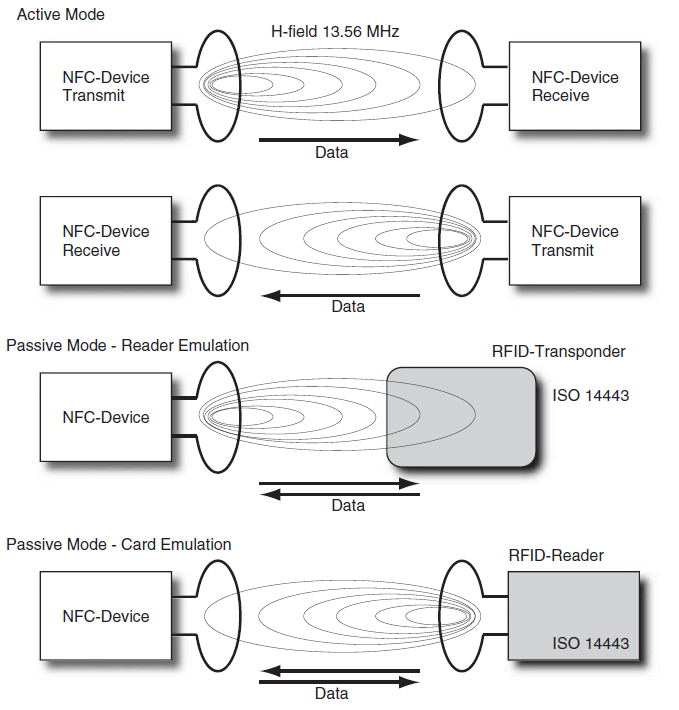
\includegraphics[width=0.6\textwidth]{images/nfc_communication}
		\vspace*{0pt}
	\caption[NFC operating modes]{NFC operating modes \citep[p.~58]{Finkenzeller.2010}}
	\label{fig:nfc_communication}
\end{figure}

\lipsum[2]

\begin{equation}
	\overline{x} = \frac 1n \sum^n_{i=1} x_i
\end{equation}

\lipsum[2] 

My reference to Tabelle~\ref{tbl:beispieltabelle1}.

% Zur Generierung von Tabellen kann das Excel-Plugin "Excel2Latex" verwendet werden
\begin{table}
	\centering
	
		\begin{tabular}{|l|l|r|}
		\hline
			\textbf{Farbe} & \textbf{Form} & \textbf{Zahl} \\
		\hline
			Rot & Rechteck & 100 \\
		\hline
			Blau & Kreis & 99 \\
		\hline
			Gelb & Dreieck & 98 \\
		\hline
		\end{tabular}
		\caption{Another table layout}
	    \label{tbl:beispieltabelle1}
	
\end{table}

\subsection{Unterunterkapitel 2}

\section{Unterkapitel 2}

\section{Unterkapitel 3}
    \chapter{Blockchain 2.0}
\section{Probleme von Bitcoin und Erweiterung der Konzepte durch Ethereum}
\section{Theoretische Grundlagen von Ethereum}
    \chapter{Blockchain im Online Advertising}
\section{Wie Online Advertising funktioniert}
\section{Mögliche Verbesserungen mittels Blockchain-Technologie}
\section{Programmierung eines geeigneten Smart Contracts in Solidity}
\section{Beantwortung der Forschungsfrage}
\section{Blockchain 3.0 - Bestehende Probleme und potenzielle Lösungen}
        \include{chapter05}
    
\appendix
\chapter{Anhang}
Lorem ipsum dolor sit amet, consectetuer adipiscing elit. Cras semper. Integer sapien nulla, consectetuer a, laoreet et, varius quis, mauris. Nunc pharetra tincidunt massa. Pellentesque habitant morbi tristique senectus et netus et malesuada fames ac turpis egestas. Praesent pellentesque mauris at elit. Aliquam consequat suscipit enim. Pellentesque habitant morbi tristique senectus et netus et malesuada fames ac turpis egestas. Nunc sapien. Proin hendrerit diam at quam. Lorem ipsum dolor sit amet, consectetuer adipiscing elit. Integer vulputate semper nunc. Sed dui. Praesent at sem. Integer elit ipsum, placerat vitae, dictum quis, feugiat sit amet, metus.

\section{Anhang A}
Donec arcu turpis, pretium quis, interdum non, condimentum a, est. Fusce lobortis urna non tellus. Nam leo dui, malesuada non, tempus placerat, congue eget, pede. Mauris porttitor risus quis tortor molestie vehicula. Curabitur tincidunt. In malesuada congue nisi. Nullam et nulla. Curabitur porttitor. Ut molestie sagittis felis. Sed urna libero, ultricies quis, laoreet eget, congue id, metus. Proin ac lorem cursus mauris auctor laoreet. Donec justo. Etiam nunc sem, dapibus sit amet, euismod a, molestie sit amet, mi.

Morbi sollicitudin consequat magna. Vivamus dictum. Nulla non quam. Nam sem tellus, aliquam sed, hendrerit nec, imperdiet ut, augue. Aliquam erat volutpat. Vivamus non ligula sit amet lorem accumsan viverra. Cras mattis libero et ante. Cras massa. Donec fringilla, metus vitae semper condimentum, dolor dui fringilla arcu, et mattis nulla dui vel lectus. Nunc mauris magna, tristique eu, rutrum at, facilisis eu, odio. Nullam congue magna non nisi. Suspendisse viverra, massa non pellentesque scelerisque, risus elit 

\noindent Hier kommt ein Listing \ref{lst:soap}.

\begin{center}
\begin{lstlisting}[caption={SOAP Anfrage an einen HalloWelt-Web-Service},captionpos=b,language=XML,label={lst:soap}]
<?xml version='1.0' encoding='UTF-8'>
<SOAP-ENV:Envelope (*@\label{lst:soapEnv}@*)
  xmlns:SOAP-ENV="http://schemas.xmlsoap.org/soap/envelope/"
  xmlns:xsi="http://www.w3.org/2001/XMLSchema-instance"
  xmlns:xsd="http://www.w3.org/2001/XMLSchema"
  xmlns:ns1="http://localhost/wsdl/HalloWeltService.wsdl">
  
  <SOAP-ENV:Body>(*@\label{lst:soapBody}@*)
  	<ns1:gruss>
  		<name xsi:type="xsd:string">
  			Michael
  		</name>
  	</ns1:gruss>
  </SOAP-ENV:Body>

</SOAP-ENV:Envelope>
\end{lstlisting}
\end{center}

bibendum dolor, vitae ultrices lorem neque et erat. Nullam tortor ante, venenatis et, aliquet ac, ornare id, massa. Vivamus urna augue, posuere vitae, sagittis id, porttitor at, arcu. Praesent pharetra rutrum neque. Maecenas tempor ultrices felis.
Nulla facilisi. In sed elit aliquet neque malesuada blandit. Nam tempus imperdiet eros. Mauris tincidunt diam eu erat. Phasellus iaculis blandit leo. Nunc augue. Donec dignissim accumsan pede. Ut consequat, eros id accumsan placerat, mi justo ullamcorper pede, id lacinia augue nisi non nibh. Vestibulum eget arcu. Cras pretium, dui eu gravida varius, lectus neque accumsan ligula, eu sodales magna lectus ut nisi. Aliquam vel ante. Ut suscipit porta augue. Suspendisse pellentesque faucibus nisl. Nulla magna tortor, cursus quis, varius quis, hendrerit ut, neque.


    \cleardoublepage
    
    \urlstyle{same}
    \bibliographystyle{chicagog}
    \begingroup
    \interlinepenalty=10000
    \hyphenpenalty=105000
    \exhyphenpenalty=105000
   
   \addcontentsline{toc}{chapter}{Bibliography}
    \bibliography{thesis}
    \endgroup
    \cleardoublepage

    % Please DO NOT change the declaration (even it is in German)
    % *************************************************************************
% *    IWI Hamburg / Prof. Dr. Stefan Voß
% *    Thesis / Dissertation Latex Template                                        
% *    
% *    Author: Leonard Heilig <leonard.heilig@uni-hamburg.de>
% *   
% *    Note: some parts of this template are based on the VSIS template
% *              of Michael von Riegen <riegen@informatik.uni-hamburg.de>
% *   
% *************************************************************************
\chapter*{Eidesstattliche Versicherung}

\thispagestyle{empty}
\addcontentsline{toc}{chapter}{Eidesstattliche Versicherung}

Hiermit versichere ich an Eides statt, dass ich die vorliegende Arbeit im Studiengang \courseOfStudies ~selbstständig verfasst und keine anderen als die angegebenen Hilfsmittel -- insbesondere keine im Quellenverzeichnis nicht benannten Internet-Quellen – benutzt habe. Alle Stellen, die wörtlich oder sinngemäß aus Veröffentlichungen entnommen wurden, sind als solche kenntlich gemacht. Ich versichere weiterhin, dass ich die Arbeit vorher nicht in einem anderen Prüfungsverfahren eingereicht habe und die eingereichte schriftliche Fassung der auf dem elektronischen Speichermedium entspricht.


\vspace{1.5cm} 

\noindent Hamburg, den \uline{~~~~~~~~~~~~~~~~~~~~~~~~~~~~~~~~~~~~~~~~~~~}~~~~~~~~~~~
~~Unterschrift: \uline{~~~~~~~~~~~~~~~~~~~~~~~~~~~~~~~~~~~~~~~~~~~~~~~~~~~} 


\cleardoublepage

\newpage

% empty page
\begin{titlepage}
\mbox{}
\end{titlepage}

\end{document}

